\newcommand*{\xMin}{0}
\newcommand*{\xMax}{14}
\newcommand*{\yMin}{0}
\newcommand*{\yMax}{6}




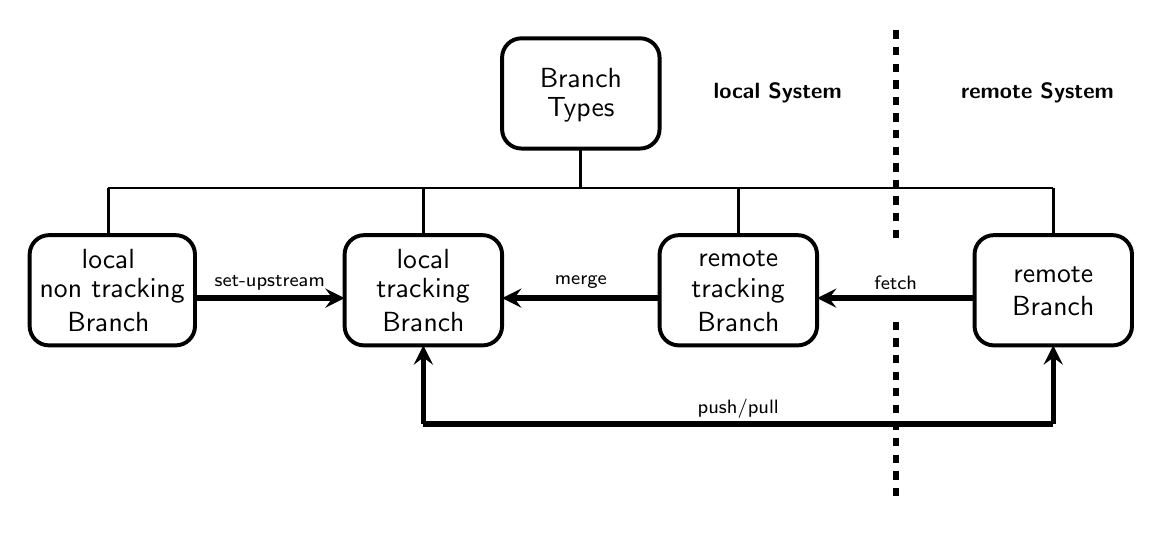
\begin{tikzpicture}
%			 \foreach \i in {\xMin,...,\xMax} {
%						\draw [very thin,gray] (\i,\yMin) -- (\i,9)  node [below] at (\i,\yMin) {$\i$};
%					}
%			\foreach \i in {\yMin,...,9
%					} {
%						\draw [very thin,gray] (\xMin,\i) -- (\xMax,\i) node [left] at (\xMin,\i) {$\i$};
%					}
		
	\node[] at(9.5,8.2) {\textbf{{\footnotesize \textsf{local System}}}};
	\node[] at(12.8,8.2) {\textbf{{\footnotesize \textsf{remote System}}}};
	
	
	% rectangle abstract branch
	\draw[line width=0.5mm,rounded corners=7pt](6,7.5) rectangle ++(2.0,1.4);
	\node[] at(7,8.4) {\textsf{Branch}};
	\node[] at(7,8.0) {\textsf{Types}};
	
	% rectangle local non tracking branch
	\draw[line width=0.5mm,rounded corners=7pt](0.0,5.0) rectangle ++(2.1,1.4);
	\node[] at(1.0,6.1) {\textsf{local}};
	\node[] at(1.05,5.7) {\textsf{non tracking}};
	\node[] at(1.0,5.3) {\textsf{Branch}};
	
	% rectangle local tracking branch
	\draw[line width=0.5mm,rounded corners=7pt](4.0,5.0) rectangle ++(2.0,1.4);
	\node[] at(5.0,6.1) {\textsf{local}};
	\node[] at(5.0,5.7) {\textsf{tracking}};
	\node[] at(5.0,5.3) {\textsf{Branch}};
	
	% rectangle remote tracking branch
	\draw[line width=0.5mm,rounded corners=7pt](8.0,5.0) rectangle ++(2.0,1.4);
	\node[] at(9.0,6.1) {\textsf{remote}};
	\node[] at(9.0,5.7) {\textsf{tracking}};
	\node[] at(9.0,5.3) {\textsf{Branch}}; 
	
	% rectangle remote branch
	\draw[line width=0.5mm,rounded corners=7pt](12,5.0) rectangle ++(2.0,1.4);	
	\node[] at(13.0,5.9) {\textsf{remote}};
	\node[] at(13.0,5.5) {\textsf{Branch}};
	
	% connection lines
	\draw[line width=1.0pt] (7.0,7.5) -- (7.0,7.0);
	\draw[line width=1.0pt] (1.0,7.0) -- (1.0,6.4);
	\draw[line width=1.0pt] (5.0,7.0) -- (5.0,6.4);
	\draw[line width=1.0pt] (9.0,7.0) -- (9.0,6.4);
	\draw[line width=1.0pt] (13.0,7.0) -- (13.0,6.4);
	\draw[line width=1.0pt] (1.0,7.0) -- (13.0,7.0);
	
	% arrows
	\draw[-stealth,line width=2pt](2.1,5.6) -- (4.0,5.6);
	\node[] at(3.05,5.8) {{\scriptsize\textsf{set-upstream}}};
	
	\draw[stealth-,line width=2pt](6.0,5.6) -- (8.0,5.6);
	\node[] at(7.0,5.8) {{\scriptsize\textsf{merge}}};
	
	\draw[stealth-,line width=2pt](10.0,5.6) -- (12.0,5.6);
	\node[] at(11.0,5.8) {{\scriptsize\textsf{fetch}}};
	
	\draw[stealth-,line width=2pt](5.0,5.0) -- (5.0,4.0);
	\draw[stealth-,line width=2pt](13.0,5.0) -- (13.0,4.0);
	\draw[line width=2pt] (5.0,4.0) -- (13.0,4.0);
	\node[] at(9.0,4.2) {{\scriptsize\textsf{push/pull}}};
	
	% dashed line
	\draw[dashed,line width=2pt] (11.0,5.3) -- (11.0,3.0);
	\draw[dashed,line width=2pt] (11.0,9.0) -- (11.0,6.3); 
	
	% commit tree
%	\draw[line width=1.0pt] (1,3.5) circle (6mm);
%	\node[] at(1,3.5) {\textsf{C1}};
%	\draw[line width=2.0pt] (1.6,3.5) -- (2.4,3.5);
%	\draw[line width=1.0pt,fill=pastelorange] (3,3.5) circle (6mm);
%	\node[] at(3,3.5) {\textsf{C2}};
%	\draw[-stealth,line width=2pt](3,2.1) -- (3,2.86);
%	\node[] at(3.0,1.9) {\textbf{{\footnotesize \textsf{master}}}};
%	\node[] at(3.0,1.6) {\textbf{{\footnotesize \textsf{HEAD}}}};
%	\node[] at(3.0,1.25) {\textbf{{\footnotesize \textsf{(new)}}}};
%	\draw[line width=1.0pt] (12.5,3.5) circle (6mm);
%	\node[] at(12.5,3.5) {\textsf{C3}};
%	\draw[-stealth,line width=2pt](12.5,2.1) -- (12.5,2.86);
%	\node[] at(12.5,1.9) {\textbf{{\footnotesize \textsf{master}}}};
%	\node[] at(12.5,1.6) {\textbf{{\footnotesize \textsf{HEAD}}}};
%	\node[] at(12.5,1.25) {\textbf{{\footnotesize \textsf{(old)}}}}; 
%	
%	\draw[stealth-,dashed,line width=1.0pt] (3.6,2.5) -- (11.9,2.5);
%	\node[] at(7.5,2.75) {\textbf{{\footnotesize \textsf{move pointer}}}}; 
%	\draw[-{Implies},double, line width=1.5pt] (12.4,4.5) -- (12.0,5.8);
	
\end{tikzpicture}